
%(BEGIN_QUESTION)
% Copyright 2008, Tony R. Kuphaldt, released under the Creative Commons Attribution License (v 1.0)
% This means you may do almost anything with this work of mine, so long as you give me proper credit

If a set of six electromagnet coils were spaced around the periphery of a circle and energized by 3-phase AC power, and a magnetic compass were placed in the center of that circle, the compass needle would rotate because it would experience a rotating magnetic field produced by these coils:

$$\includegraphics[width=15.5cm]{i01443x01.eps}$$

Explain why the magnetic field produced by the stator coils appears to rotate, and also calculate the rotational speed of this field if the 3-phase AC power frequency is 60 Hz.  Based on the rotation shown (by the arrows), what is the {\it phase sequence} of the AC power applied to the motor?

\vskip 10pt

Also, determine what would have to be changed in this scenario for the compass needle to spin at only {\it half} the speed it does now.

\vskip 10pt

Also, determine what would have to be changed in this scenario for the compass needle to spin in the {\it reverse direction} as it does now.

\vskip 20pt \vbox{\hrule \hbox{\strut \vrule{} {\bf Suggestions for Socratic discussion} \vrule} \hrule}

\begin{itemize}
\item{} Why does a real three-phase motor have its three phase coils built in pairs, as is shown here?  Why not just have three coils instead of six?
\item{} Suppose that one of the lines in the three-phase power source feeding this motor were to fail open, preventing current through one of the sets of coils in the stator of this motor.  Would the compass needle still spin?  Why or why not?
\item{} What would the stator coil arrangement look like for a {\it four} phase electric motor?
\end{itemize}

\underbar{file i01443}
%(END_QUESTION)





%(BEGIN_ANSWER)

It is helpful to recall how three-phase power is {\it generated} when trying to answer this question: we generate three-phase power by rotating a magnet at the center of three sets of coils, spaced 120$^{o}$ apart from each other around the circle.

\vskip 10pt

The magnetic field appears to rotate because the stator windings are energized out-of-step in a 1-2-3 sequence.  This is not unlike a string of blinking ``Christmas lights'' which appear to move because the lights blink in a sequence that has a definite direction.

\vskip 10pt

The compass needle's rotational speed would be 3600 RPM (60 revolutions per second) as a power supply frequency of 60 Hz.  To halve this speed, we would either need to add twice as many poles to the motor, or else halve the frequency (30 Hz).

\vskip 10pt

To reverse the needle's direction, reverse the phase sequence of the power.  This may be accomplished by swapping any two of the three power conductors to the stator.

%(END_ANSWER)





%(BEGIN_NOTES)


%INDEX% Final Control Elements, motor: rotating magnetic field

%(END_NOTES)


